\section{Results}
Given the facts highlighted by \cref{eq:ZsquareIntegral} and \cref{eq:SecondDerivativeIntegral}, the formula to calculate the eSTA corrections \cref{eq:eSTAcorrections} simplifies even further to
\begin{equation}
	\label{eq:eSTAcorrectionsSimplified}
	-\frac
	{
		\left( \sum_{n=1}^{\mathcal{N}} |G_{n}|^2 \right) \text{Re}(G_{2}^{*}\vec{K}_{2})
	}
	{
		\left|\text{Re}(G_{n}^{*}\vec{K}_{n})\right|^2
	}
\end{equation}
and some results are shown in the figures where the fidelity with respect to the total time of the protocols are shown for different number of particles.
In the following we tested the results we obained by applying the eSTa protocols to two different Hamiltonians:
\begin{itemize}
	\item The Hamiltonian \cref{eq:TaylorExpansionHamiltonian} which is an approximation of the original Hamiltonian \cref{eq:DimensionlessBoseHubbardHamiltonian}
	\item The Hamiltonian \cref{eq:SchrodingerEquationCoefficientsContinuous} which is the continuous version of the exact Hamiltonian \cref{eq:DimensionlessBoseHubbardHamiltonian}
\end{itemize}
The results show that in any cases the eSTA protocol produces an improvement on the respective STA one and in particular we can see that  the improvement is more prominent when we use the full version of the Bose Hubbard Hamiltonian with no approximations involved.
\begin{figure}[t]
	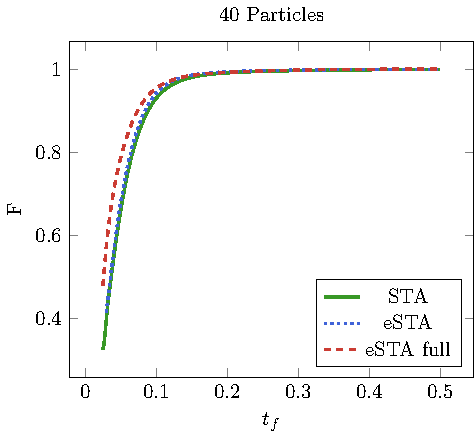
\includegraphics[width = \textwidth]{gfx/fidelity_compare_40.pdf}
	\caption{Comparison between the fidelity for 40 particles and for different final times, we can see eSTA outperforming the STA counterparts in both cases and it is more noticeable when eSTA is applied to the original version of the Bose Hubbard Hamiltonian.}
	\label{fig:FidelityCompare40}
\end{figure}
\begin{figure}[t]
	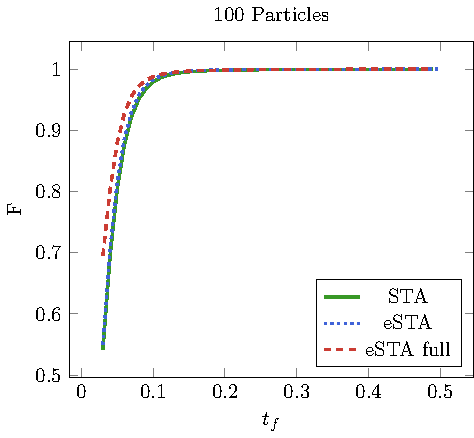
\includegraphics[width = \textwidth]{gfx/fidelity_compare_100.pdf}
	\caption{Similar comparison with 100 particles, again the figure shows the best performances obtained using eSTA. We can also see how the approximation is more stable for smaller final times when compared to the other figure with less particles.}
	\label{fig:FidelityCompare100}
\end{figure}
